\section*{\hfil Структура проекта\hfil}

%\noindent\hrulefill
%\begin{figure}[H]
%	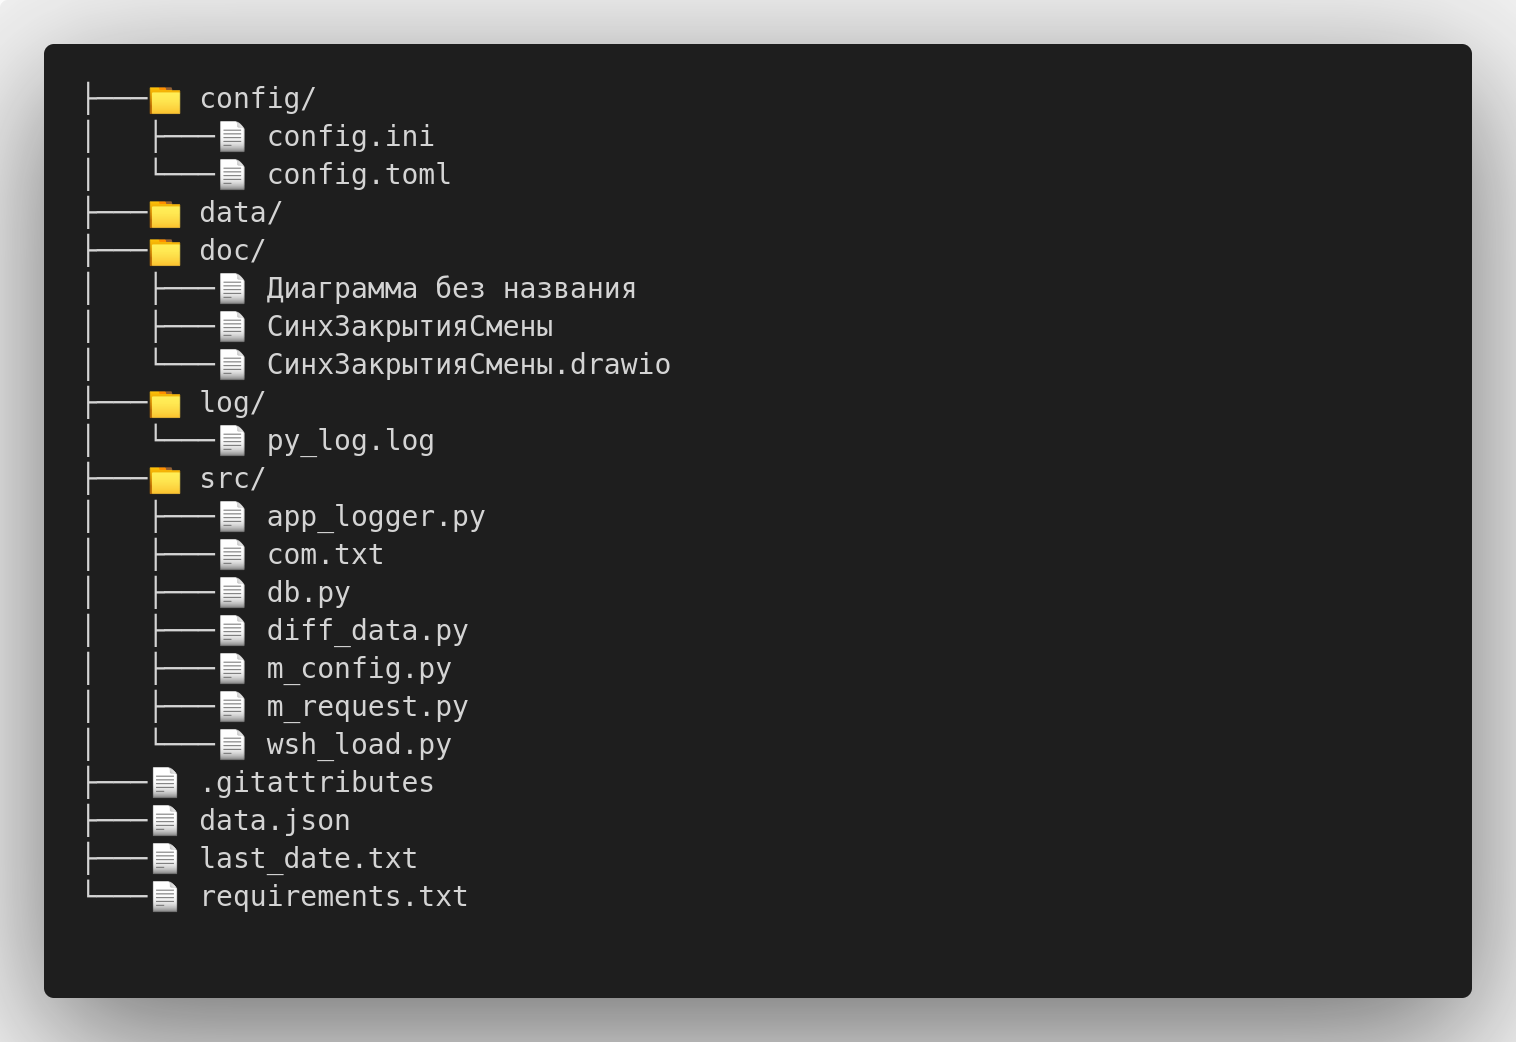
\includegraphics[width=0.95\textwidth]{code.png}
%	\caption{<<Структура проекта>>.}
%	\label{ris:code.png}
%\end{figure}

\renewcommand*\DTstylecomment{\rmfamily\color{blue}\sffamily}
\renewcommand*\DTstyle{\ttfamily\textcolor{black}}
\setlength{\DTbaselineskip}{20pt}
%\DTsetlength{1em}{3em}{0.1em}{1pt}{4pt}

\dirtree{%
	.1 /.	
	.1 Workshift\_load.
	.2 config.\DTcomment{каталог с файлами настроек}.
	.3 config.ini\ldots{} \begin{minipage}[t]{5cm}
		Файл содержит настройки программы{.}
	\end{minipage}.
	.2 log.\DTcomment{каталог с файлами лога}.
	.3 py\_log.log\DTcomment{файл лога}.
	.2 src.\DTcomment{каталог с файлами программы}.
	.3 app\_logger.py.\DTcomment{работа с логированием}.
	.3 db.py.\DTcomment{Работа с БД}.	
	.3 diff\_data.py.\ldots{} \begin{minipage}[t]{5cm}
		Файл содержит тексты запросов{.}
	\end{minipage}.
	.3 m\_config.py.\DTcomment{работа с конфигурацией}.	
	.3 m\_request.py.\DTcomment{работа с Http-запросами}.		
	.3 wsh\_load.py.\DTcomment{основной файл программы}.				
	.3 last\_date\_open.txt.\DTcomment{дата последней открытой смены ККМ}.	
	.3 last\_date.txt.\DTcomment{дата последней закрытой смены ККМ}.	
	.3 first.dat.\ldots{} \begin{minipage}[t]{5cm}
		Файл появляется после первого запуска программы
		если он отсутствует, то при запуске происходит 
		инициализация файлов с датами смен ККМ{.}
	\end{minipage}.
	.1 requirements.txt.\ldots{} \begin{minipage}[t]{5cm}
		Файл содержит наименование и версии установленных 
		модулей подключенных к программе, используется
		при начальной установке{.}
	\end{minipage}.
}
\newpage

\section{Алгоритм}

\begin{itemize}

\item При запуске программы производится проверка на наличие в каталоге <<src>> файла
<<first.dat>>. Если он не обнаружен это считается первым запуском программы и вызывается процедура инициализации, которая создает два текстовых файла с датами равными началу года. Таким образом при первом запуске по запросу с этими заведомо ранними датами, в результат запроса попадут \textbf{все} кассовые смены имеющиеся в Artix, а даты в файлах будут установлены на максимальное значение открытия и закрытия смен.
\newline


	\begin{lstlisting}[language=Python, label=some-code,caption=Инициализация файлов с датами]
def init_pr():

	filename = '/home/administrator/Workshift_load/src/last_date.txt'
	if not os.path.exists(filename):
		with open(filename, 'w', encoding='utf-8') as outfile:
			outfile.write('2023-01-01 00:00:00')

	filename = '/home/administrator/Workshift_load/src/last_date_open.txt'
	if not os.path.exists(filename):
		with open(filename, 'w', encoding='utf-8') as outfile:
			outfile.write('2023-01-01 00:00:00')
			   	\end{lstlisting}


	
\item При запуске программы происходит чтение настроек. Если чтение удачно, запускается функция <<main()>>, в противном случае программа завершает свою работу.
\newline

%\begin{figure}[H]
%	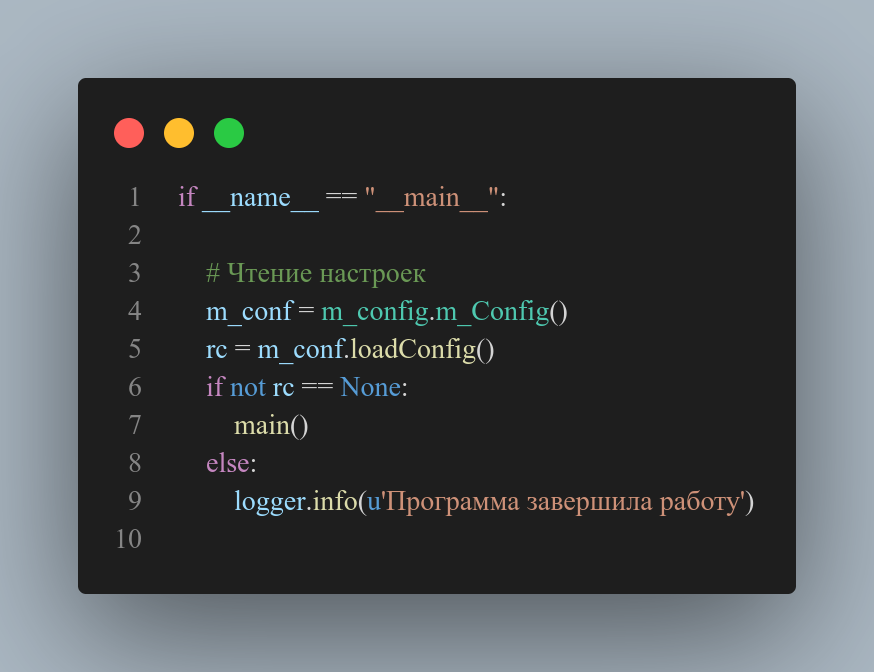
\includegraphics[width=0.65\textwidth]{code1.png}
%	\caption{<<Структура проекта>>.}
%	\label{ris:code1.png}
%\end{figure}



	\begin{lstlisting}[language=Python, caption=Начало работы]
if __name__ == "__main__":

	# Чтение настроек
	m_conf = m_config.m_Config()   
	rc =  m_conf.loadConfig()
	if not rc == None:
		main()
	else:
		logger.info(u'Программа завершила работу') 
	\end{lstlisting}


\newpage

Настройки хранятся в файле \path{/config/config.ini} . Примерный вариант файла настроек:


   \begin{lstlisting}[language={Ini}]
	; comment1
	[artix]
	path = world
	tPriceQR = 1
	server_ip = 192.168.0.239
	exchange_cat = //192.168.0.239/obmen/dict/
\end{lstlisting}

\item При запуске функции <<main()>> происходит соединение с базой данных и создается объект для работы с ней. Работа с БД осуществляется в файле <<db.py>>
Создаем экземпляр класса "<workDb"> для работы с базой данных предавая в качестве параметра при инициализации объект содержащий текущие настройки программы полученные из "<ini"> файла.
\newline
	\begin{lstlisting}[language=Python, caption=Создание объекта БД]
    tData = db.workDb(rc)
	\end{lstlisting}


При инициализации происходит подключение к БД и возвращается текущий курсор.
В качестве параметров строка подключения содержит: IP-адрес сервера, имя БД, имя и пароль пользователя.
\newline
	\begin{lstlisting}[language=Python, caption=Соединение с БД]
self.mydb = pymysql.connect(host=rc._sections.artix.server_ip,......"IP-адрес сервера"
							database=rc._sections.artix.database,............"имя БД"
							user=rc._sections.artix.user,.........................."имя пользователя"
							passwd=rc._sections.artix.passwd)................."пароль"
self._mycursor = self.mydb.cursor()  # cursor created
	\end{lstlisting}




%	
Так же создается объект для работы с Http запросами.


	\begin{lstlisting}[language=Python, caption=Объект запрос]
	rec_con = m_request.req1C(rc)
		\end{lstlisting}


\item Получаем список смен которые были открыты с последней зафиксированной даты.

	\begin{lstlisting}[language=Python, caption=Список открытых смен]
	# Список открытых смен от последнего зафиксированного времени
	l_workshift_open = tData.get_last_workshift_open()
	\end{lstlisting}

\newpage
Получение списка открытых смен с момента последнего обращения к БД
\newline
	\begin{lstlisting}[language=Python, caption=Смены из БД]
	# Читаем из файла дату открытия последней отправленной в УНФ смены
	l_date = self.load_last_date_open()

	# Выполняем запрос с отбором по дате
	# Текст запроса хранится в файле "diff_data.py"
	
	# "'SELECT shiftnum ,cashcode,CAST(time_beg AS char),shopcode  FROM workshift WHERE time_end IS NULL AND time_beg >%s  '"
	
	self._mycursor.execute(diff_data.qrSelect_workshift_open, [l_date])

	# Результат выполнения запроса
	l_workshift = self._mycursor.fetchall()
		\end{lstlisting}


 Если появились новые открытые смены, тогда формируем и отправляем Http запрос в 1С. 
\newline
\begin{lstlisting}[language=Python, caption=Http-запрос]
	status_code = rec_con.post_workshift_open(l_workshift_open)
\end{lstlisting}
С запросами работает файл "<m\_request.py"> 
\newline
\begin{lstlisting}[language=Python, caption=Текст Http-запроса]
	r = requests.post('http://' + self.mConfig._sections.one_C.server_ip + ':'..... IP адрес 
						+ self.mConfig._sections.one_C.port........................................Port
						+ self.mConfig._sections.one_C.workshift_open,.................... Процедура
						 data=None, json = l_workshift_open)................................... Данные смен ККМ
	return (r.status_code)
\end{lstlisting} 
 
В 1С данные отправляются в виде списка со значениями. Пример файла:

\begin{lstlisting}[language=json,firstnumber=1, caption= Формат файла открытых смен]
97, ..................................... Номер смены
'test', ................................. Код кассы
'2023-02-06 13:35:38', ........ Дата открытия
'test' .................................. Код магазина
\end{lstlisting}
 
\newpage 
 
Если код возврата был успешным (\textbf{200}), тогда меняем дату в файле, на дату открытия последней смены.
\newline

	\begin{lstlisting}[language=Python, caption=Обработка результата]
 # Список открытых смен от последнего зафиксированного времени
	l_workshift_open = tData.get_last_workshift_open()
	# Если нечего отправлять, то не отправляем
	if len(l_workshift_open) > 0:
		status_code = rec_con.post_workshift_open(l_workshift_open)
	# Меняем дату в файле только в случае успешного результата работы 1C
		if status_code == 200:
			tData.save_new_date_open()
		else:
			logger.info('status_code_open - ' + str(status_code ))
	\end{lstlisting}



\item Получаем список смен которые были закрыты с последней зафиксированной даты, если появились новые закрытые смены, тогда формируем и отправляем Http запрос в 1С. 


В 1С данные отправляются в виде списка со значениями. Пример файла:

\begin{lstlisting}[language=json,firstnumber=1, caption= Формат файла закрытых смен]
96,.................................. ... Номер смены
'test', ................................. Код магазина
'2023-02-06 13:33:40', ....... Дата открытия 
'test', ................................. Код кассы
'2023-02-03 10:02:25', ........ Дата закрытия
103, ................................... Идентификационный номер смены
'_shop_test_56f60925', .... storeId
'_cash_test_e0146422', .... cashId
'3', ..................................... Код кассира
1, ....................................... Номер первого чека смены
3, ....................................... Номер последнего чека смены
'637.0000', ......................... Сумма продажи
'637.0000',  ........................ Сумма выручки
'637.0000',  ........................ Сумма в денежном ящике
'2023-02-03 10:02:22',  ....... Дата и время открытия первого чека в смене
'637.00', ............................. Сумма продажи (наличные)
'0.00',  ................................ Сумма продажи (безналичные)
'0.00',  ................................ Сумма продажи (прочие)
'637.00', ............................. Сумма выручки (наличные)
'0.00',  ................................ Сумма выручки (безналичные)
'0.00',  ................................ Сумма возвратов
'0.00', ................................. Сумма возвратов (наличные)
'0.00', ................................. Сумма возвратов (безналичные)
3,  ....................................... Количество чеков продажи
0  ........................................ Количество чеков возврата
\end{lstlisting}



Если код возврата был успешным (\textbf{200}), тогда меняем дату в файле, на дату закрытия последней смены.
\newline
	\begin{lstlisting}[language=Python, caption=Закрытые смены]
	# Список закрытых смен от последнего зафиксированного времени
	l_workshift = tData.get_last_workshift()
	# Если нечего отправлять, то и  не отправляем
	if len(l_workshift) > 0:
		status_code = rec_con.post_workshift(l_workshift)
	# Меняем дату в файле только в случае успешного результата работы 1C
		if status_code == 200:
			tData.save_new_date()
		else:
			logger.info('status_code_open - ' + str(status_code ))
	\end{lstlisting}


\item Завершаем работу программы.




\end{itemize}

\newpage
